\section*{Исходные данные}

\begin{table}[H]
	\renewcommand{\tablename}{Таблица}
	\caption{Интенсивности поступления потоков обслуживаемых процессов}
	\begin{tabularx}{1\textwidth}{
			| >{\centering\arraybackslash}X
			| >{\centering\arraybackslash}X
			| >{\centering\arraybackslash}X
			| >{\centering\arraybackslash}X
			| >{\centering\arraybackslash}X
			| >{\centering\arraybackslash}X
			| >{\centering\arraybackslash}X
			| >{\centering\arraybackslash}X
			| >{\centering\arraybackslash}X
			| >{\centering\arraybackslash}X
			| >{\centering\arraybackslash}X |
		}
		\hline
		\multirow{2}{*}{\rotatebox[origin=c]{90}{№ варианта}} & \multirow{2}{*}{\rotatebox[origin=c]{90}{№ потока}} & \rotatebox[origin=c]{90}{Интенсивность потока} & \multirow{2}{*}{\rotatebox[origin=c]{90}{№ потока}} & \rotatebox[origin=c]{90}{Интенсивность потока} & \multirow{2}{*}{\rotatebox[origin=c]{90}{№ потока}} & \rotatebox[origin=c]{90}{Интенсивность потока} & \multirow{2}{*}{\rotatebox[origin=c]{90}{№ потока}} & \rotatebox[origin=c]{90}{Интенсивность потока} & \multirow{2}{*}{\rotatebox[origin=c]{90}{№ потока}} &
		\rotatebox[origin=c]{90}{Интенсивность потока} \\
		\cline{3-3}\cline{5-5}\cline{7-7}\cline{9-9}\cline{11-11}
		& & [1/c] & & [1/c] & & [1/c] & & [1/c] & & [1/c] \\
		\hline
		7 & 7 & 0,20 & 14 & 0,40 & 10 & 0,05 & 19 & 0,05 & 1 & 0,20\\
		\hline
	\end{tabularx}\label{tab:table2}
\end{table}

\begin{table}[H]
	\renewcommand{\tablename}{Таблица}
	\caption{Параметры обслуживаемых процессов.}
	\begin{tabularx}{1\textwidth}{
			| >{\centering\arraybackslash}p{1cm} | >{\centering\arraybackslash}p{5.7cm} | >{\centering\arraybackslash}p{0.5cm} | >{\centering\arraybackslash}p{0.5cm} | >{\centering\arraybackslash}p{0.5cm} | >{\centering\arraybackslash}p{0.5cm} | >{\centering\arraybackslash}p{0.5cm} | >{\centering\arraybackslash}p{0.5cm} | >{\centering\arraybackslash}p{0.5cm} | >{\centering\arraybackslash}p{0.5cm} | >{\centering\arraybackslash}p{0.5cm} | >{\centering\arraybackslash}p{0.5cm} |
		}
		\hline
		\multirow{3}{1cm}{№ процесс
			а} & 
		\multirow{3}{6cm}{Среднее количество вычислительных 
			операций, выполняемых 
			при обслуживаниях процесса 
			[Мфлоп] } & 
		\multicolumn{10}{X|}{Среднее число операций обращения к файлам данных при обслуживании процесса (N i j) }
		\\
		\cline{3-12}
		& &  \multicolumn{10}{X|}{Номера файлов, к которым выполняется обращение} \\
		\cline{3-12}
		& & F1 & F2 & F3 & F4 & F5 & F6 & F7 & F8 & F9 & F10 \\ \hline
		7 & 700 & 20 & - & - & 10 & - & - & 2 & - & 4 & - \\ \hline
		14 & 400 & 10 & - & 30 & 14 & - & - & 4 & - & 6 & - \\ \hline
		10 & 1000 & - & 30 & - & - & - & 20 & 6 & - & 8 & - \\ \hline
		19 & 900 & - & 80 & - & 30 & - & - & 8 & - & - & 4 \\ \hline
		1 & 100 & 20 & 10 & - & - & - & - & 4 & 2 & - & - \\ 
		\hline
	\end{tabularx}\label{tab:table1}
\end{table}

\begin{table}[H]
	\renewcommand{\tablename}{Таблица}
	\caption{Интенсивности поступления потоков обслуживаемых процессов}
	\begin{tabularx}{1\textwidth}{
			| >{\centering\arraybackslash}X
			| >{\centering\arraybackslash}X
			| >{\centering\arraybackslash}X |
		}
		\hline
		№ файлов данных & Объем данных, передаваемых при выполнении одной операции 
		обращения к файлу данных 
		V FI [Мбайт] & Средний объем данных, передаваемых при выполнении одной операции ввода/вывода 
		G FI [Кбайт] \\
		\hline
		F1 & 0,5 & 5 \\ \hline
		F2 & 1,0 & 8 \\ \hline
		F3 & 1,0 & 15 \\ \hline
		F4 & 1,5 & 6 \\ \hline
		F5 & 1,5 & 14 \\ \hline
		F6 & 2,0 & 18 \\ \hline
		F7 & 2,5 & 10 \\ \hline
		F8 & 3,0 & 15 \\ \hline
		F9 & 4,0 & 20 \\ \hline
		F10 & 0,5 & 5 \\ \hline
	\end{tabularx}\label{tab:table}
\end{table}

\begin{table}[H]
	\renewcommand{\tablename}{Таблица}
	\caption{Характеристики накопителей внешней памяти.}
	\begin{tabularx}{1\textwidth}{
			| >{\centering\arraybackslash}p{3cm}
			| >{\centering\arraybackslash}p{6cm}
			| >{\centering\arraybackslash}p{6cm} |
		}
		\hline
		\multirow{3}{*}{№ файла данных}  & \multicolumn{2}{X|}{\centering{Среднее время выполнения одной операции ввода/вывода данных    [мкc/ оп.]}}  \\
		\cline{2-3}
		& \multicolumn{2}{X|}{\centering{Тип накопителя ВЗУ, на котором размещены файлы данных}} \\
		\cline{2-3}
		& НМД 1 & НМД 2 \\ \hline
		F1 & 1,0 & - \\ \hline
		F2 & - & 0,10 \\ \hline
		F3 & 2,0 & - \\ \hline
		F4 & - & 0,05 \\ \hline
		F5 & 3,0 & - \\ \hline
		F6 & - & 0,06 \\ \hline
		F7 & 2,5 & - \\ \hline
		F8 & - & 0,13 \\ \hline
		F9 & 2,5 & - \\ \hline
		F10 & - & 0,12 \\ \hline
	\end{tabularx}\label{tab:table4}
\end{table}


\subsection*{Ход работы}

\subsubsection*{Модель M1}

При обслуживании в однопроцессорной системе M независимых потоков процессов с примерно одинаковой сложностью обслуживания и при использовании в качестве дисциплины планировании дисциплины FIFO (Fitst In First Out) время ожидания любого процесса из M потоков процессов примерно одинаково и определяется по выражению (\ref{fig:m1})

\begin{align}
	\omega = \sum_{i=1}^{M}\frac{\lambda_i\vartheta_i(1+v^2_i)}{2(1-R)}
	\label{fig:m1}
\end{align}


где $M$ - количество процессов, поступающих но обслуживание в систему, \\
$R = (\rho_1 + \rho_2 + \rho_3 + ... +\rho_m)$

$\rho_i$ - коэффициент загрузки ресурсов системы $i$ -- ым процессом. \\
Значение $\rho_i$ определяется по выражению (\ref{fig:m2})\\

\begin{align}
	\rho_i = \lambda_i\vartheta_i 
	\label{fig:m2}
\end{align}

где $\lambda_i$ -- интенсивность $i$ -- потока процессов на обслуживание в систему, \\
$\vartheta = (\vartheta_1,\vartheta_2,\vartheta_3,...,\vartheta_k) / k$ , \\
$\vartheta_k$ -- длительность обслуживания процесса $k$--ом ресурсе системы. \\
Длительность обслуживания процесса в $k$--ом ресурсе системы определяется по выражению \ref{formul:3}

\begin{align}
	\vartheta_{pi} =  \Theta_i/V_p
	\label{formul:3}
\end{align}

где 

$V_p$ --производительность процессора,
$\Theta_i$ -- количество вычислительных операций, выполняемых при обслуживании процесса в системе, \\

Время обслуживания одного обрушения к $j$-му файлу $i$-м процессом представлено в таблице \ref{table:5}.

\begin{table}[H]
	\renewcommand{\tablename}{Таблица}
	\caption{Время обслуживания одного процессора.}
	\begin{tabularx}{1\textwidth}{
			| >{\centering\arraybackslash}X
			| >{\centering\arraybackslash}X
			| >{\centering\arraybackslash}X
			| >{\centering\arraybackslash}X
			| >{\centering\arraybackslash}X
			| >{\centering\arraybackslash}X
			| >{\centering\arraybackslash}X
			| >{\centering\arraybackslash}X
			| >{\centering\arraybackslash}X
			| >{\centering\arraybackslash}X
			| >{\centering\arraybackslash}X |
		}
		\hline
		№ & F1 & F2 & F3 & F4 & F5 & F6 & F7 & F8 & F9 & F10 \\ \hline
		7 & 0,00205 & - & - & 0,00013 & - & - & 0,00128 & - & 0,00205 & - \\ \hline
		14 & 0,00102 & - & 0,00410 & 0,00018 & - & - & 0,00256 & - & 0,00307 & - \\ \hline
		10 & - & 0,00038 & - & - & - & 0,00014 & 0,00384 & - & 0,00410 & - \\ \hline
		19 & - & 0,00102 & - & 0,00038 & - & - & 0,000512 & - & - & 0,00005 \\ \hline
		1 & 0,00205 & 0,00013 & - & - & - & - & 0,00256 & 0,00005 & - & - \\ \hline
	\end{tabularx}\label{table:5}
\end{table}


Время обслуживания $i$-го процесса каждым ВЗУ (НДМ) представлены в таблице \ref{table:6}.

\begin{table}[H]
	\renewcommand{\tablename}{Таблица}
	\caption{Время обслуживания $i$-го процесса каждым ВЗУ.}
	\begin{tabularx}{1\textwidth}{
			| >{\centering\arraybackslash}X
			| >{\centering\arraybackslash}X
			| >{\centering\arraybackslash}X |
		}
		\hline
		№ & НДМ1 & НДМ2 \\ \hline
		7 & 0,005376 & 0,000128 \\ \hline
		14 & 0,010752 & 0,000179 \\ \hline
		10 & 0,007936 & 0,000521 \\ \hline
		19 & 0,005120 & 0,001457 \\ \hline
		1 & 0,004608 & 0,000181 \\ \hline
	\end{tabularx}\label{table:6}
\end{table}


Следующие расчёты приведены при производительности процессора $$V_\Pi = 10^5$$. Результаты расчёта максимальной длительности обслуживания $i$-го процесса представлены в таблице \ref{table:7}. Результаты расчета коэффициента загрузки $[\rho]$ ресурсов системы каждым процессом представлены в таблице \ref{table:8}.

\begin{table}[H]
	\renewcommand{\tablename}{Таблица}
	\caption{Максимальная длительность обслуживания $i$-го процесса.}
	\begin{tabularx}{1\textwidth}{
			| >{\centering\arraybackslash}X
			| >{\centering\arraybackslash}X
			| >{\centering\arraybackslash}X
			| >{\centering\arraybackslash}X
			| >{\centering\arraybackslash}X
			| >{\centering\arraybackslash}X |
		}
		\hline
		№ & 7 & 14 & 10 & 19 & 1 \\ \hline
		V & 0,01238 & 0,01475 & 0,01794 & 0,01412 & 0,00561 \\ \hline
	\end{tabularx}\label{table:7}
\end{table}


\begin{table}[H]
	\renewcommand{\tablename}{Таблица}
	\caption{Коэффициент загрузки ресурсов системы.}
	\begin{tabularx}{1\textwidth}{
			| >{\centering\arraybackslash}X
			| >{\centering\arraybackslash}X
			| >{\centering\arraybackslash}X
			| >{\centering\arraybackslash}X
			| >{\centering\arraybackslash}X
			| >{\centering\arraybackslash}X |
		}
		\hline
		№ & 7 & 14 & 10 & 19 & 1 \\ \hline
		$\rho$ & 0,00248 & 0,00590 & 0,00090 & 0,00071 & 0,00112 \\ \hline
	\end{tabularx}\label{table:8}
\end{table}


Время ожидания процессами в очереди и время их пребывания в СМО проставлены в таблице \ref{table:9}.

\begin{table}[H]
	\renewcommand{\tablename}{Таблица}
	\caption{Время ожидания в очереди и пребывания в СМО.}
	\begin{tabularx}{1\textwidth}{
			| >{\centering\arraybackslash}X
			| >{\centering\arraybackslash}X
			| >{\centering\arraybackslash}X |
		}
		\hline
		& $\omega$, сек & $u$, сек \\ \hline
		$v_i = 0$ & 0.00561 & 0,07040 \\ \hline
		$v_i = 1$ & 0,01120 & 0,07600 \\ \hline
	\end{tabularx}\label{table:9}
\end{table}


Графики зависимости времени ожидания и времени обслуживания представлены на рисунках \ref{img:1} и \ref{img:2}, соответственно.

\begin{figure}[H]
	\renewcommand{\figurename}{Рисунок}
	\centering{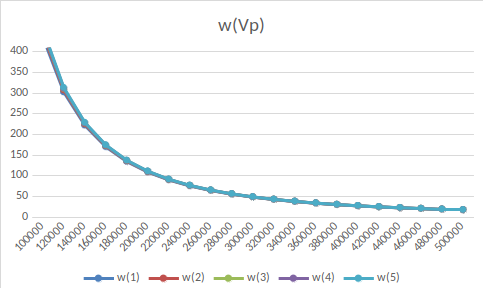
\includegraphics[scale=0.70]{img_1}}
	\caption{график зависимости $\omega(V_p)$}
	\label{img:1}
\end{figure}

\begin{figure}[H]
	\renewcommand{\figurename}{Рисунок}
	\centering{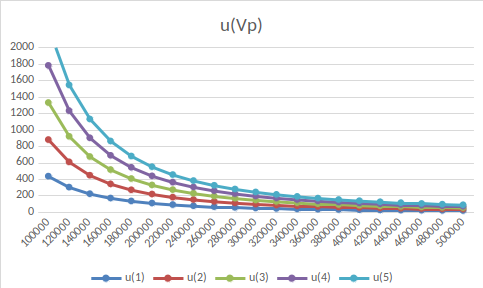
\includegraphics[scale=0.70]{img_2}}
	\caption{график зависимости $u(V_p)$}
	\label{img:2}
\end{figure}


В качестве более точной математической модели исследуемой однопроцессорной системы предлагается рассмотреть трехкомпонентную стохастическую сеть одноканальных СМО с бесприоритетной дисциплиной FIFO обслуживания очереди процессов.  В этом случае каждая из СМО сети моделирует соответствующий ресурс системы – процессор, ВЗУ1 и ВЗУ2.

Для полного определения этой модели необходимо знать вероятности переходов процессов между СМО сети при их обслуживании в системе. 

В качестве модели процесса организации обслуживания процессов в стохастической сети СМО предлагается модель, показанная на рисунке \ref{img:3}, в виде графа Маркова. 

В этом случае вероятности переходов процессов для обслуживания между СМО сети определяются по выражению (\ref{formul:4}):

\begin{align}
	p_i,_j = \frac{N_i,_j}{\sum_{i=1}^{k}N_j,_i} 
	\label{formul:4}
\end{align}

где

$N_i,_j$ -- количество переходов процесса из состояния обслуживания в $i$ -- ресурсе системы в состояние обслуживания процесса в $j$ ресурсе, \\
$\sum_{i=1}^{k}N_j,_i$ -- количество переходов процесса из состояния обслуживания в
других ресурсах системы в состояние обслуживания в $j$ ресурсе, \\
$k$ -- количество состояний моделируемой системы.

В результате определения значений $\rho_{ij}$ троится аналитическая модель обслуживания процессов в системе, представляемой системой линейных уравнений. Определяются интенсивности $\lambda_i$ поступления процессов на обслуживания в каждый модуль системы.

На рисунке \ref{img:3} представлена трёхкомпонентная стохастическая сеть одноканальной СМО. 

\begin{figure}[H]
	\renewcommand{\figurename}{Рисунок}
	\centering{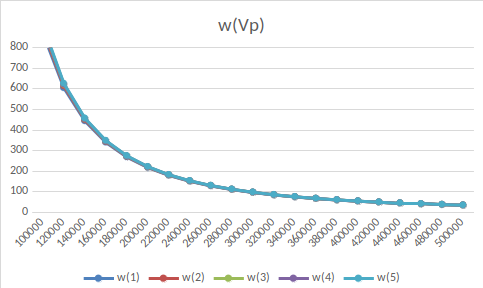
\includegraphics[scale=0.35]{img_3}}
	\caption{Трёхкомпонентная стохастическая сеть одноканальной СМО }
	\label{img:3}
\end{figure}

\begin{figure}[H]
	\renewcommand{\figurename}{Рисунок}
	\centering{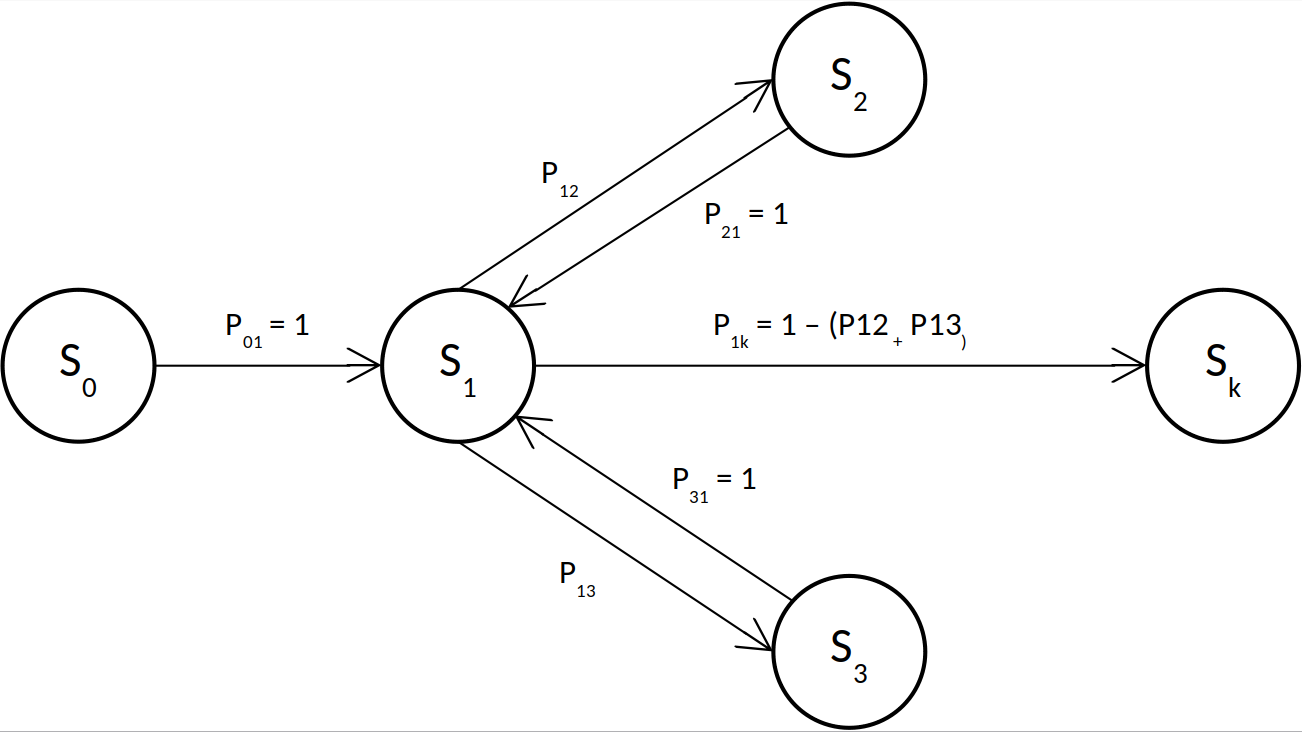
\includegraphics[scale=0.35]{img_4}}
	\caption{Модель организации обслуживания процессов }
	\label{img:4}
\end{figure}

В результате решения системы уравнений определяются интенсивности поступления процессов $\lambda_i$ на обслуживание в каждый из ресурсов системы – интенсивность поступления процессов на обслуживание в процессор, ВЗУ1 и ВЗУ2.

Определение значений интенсивностей $\lambda_i$ дает возможность выполнить более точное построение графиков зависимостей времени ожидания $\omega$ и времени обслуживания u от варьируемых параметров $\vartheta_i$ для бесприоритетной дисциплины FIFO обслуживания процессов.



Матрица переходов: 
\[
P = \begin{bmatrix}
	0 & 1 & 0 & 0 & 0 \\
	0 & 0 & P_{12} & P_{13} & P_{1k} \\
	0 & 1 & 0 & 0 & 0 \\
	0 & 1 & 0 & 0 & 0 \\
	0 & 0 & 0 & 0 & 0 \\
\end{bmatrix}
\]
Система уравнений:


$$
\lambda_1 = \lambda_0 + \lambda_2 + \lambda_3
$$
$$
\lambda_2 = \lambda_1 * P_{12}
$$
$$
\lambda_3 = \lambda_1 * P_{13}
$$
$$
\lambda_k = \lambda_1 * P_{1k} = \lambda_1 * (1-(P_{12} + P_{13}))
$$

$$
\lambda_2 = \frac{\lambda_0 * P_{12}}{1 - (P_{12} + P_{13})}
$$
$$
\lambda_3 = \frac{\lambda_0 * P_{13}}{1 - (P_{12} + P_{13})}
$$
$$
\lambda_k = \frac{\lambda_0 * 1}{1 - (P_{12} + P_{13})}
$$
$$
\lambda_k = \lambda_1 * P_{1k} = \lambda_0
$$

Матрицы переходных вероятностей

\[
P(7) = 
\begin{bmatrix}
0 & 0,70270 & 0,27027 & 0,02703 \\
1 & 0 & 0 & 0 \\
1 & 0 & 0 & 0 \\
\end{bmatrix}
\]
\[
P(14) = 
\begin{bmatrix}
0 & 0,76923 & 0,21528 & 0,01538 \\
1 & 0 & 0 & 0 \\
1 & 0 & 0 & 0 \\
\end{bmatrix}
\]
\[
P(10) = 
\begin{bmatrix}
0 & 0,21538 & 0,76923 & 0,01538 \\
1 & 0 & 0 & 0 \\
1 & 0 & 0 & 0 \\	
\end{bmatrix}
\]
\[
P(19) = 
\begin{bmatrix}
0 & 0,06504 & 0,92683 & 0,00813 \\
1 & 0 & 0 & 0 \\
1 & 0 & 0 & 0 \\
\end{bmatrix}
\]
\[
P(1) = 
\begin{bmatrix}
0 & 0,64865 & 0,32432 & 0,02703 \\
1 & 0 & 0 & 0 \\
1 & 0 & 0 & 0 \\
\end{bmatrix}
\]


Интенсивности входных потоков заявок (обращений к файлу) для СМО

\[
P(7) = 
\begin{pmatrix}
7,4 & 5,2 & 2 & 0,2\\
\end{pmatrix}
\]

\[
P(14) = 
\begin{pmatrix}
26 & 20 & 5,6 & 0,4\\
\end{pmatrix}
\]

\[
P(10) = 
\begin{pmatrix}
26 & 5,6 & 20 & 0,05\\
\end{pmatrix}
\]

\[
P(19) = 
\begin{pmatrix}
6,15 & 0,4 & 5,7 & 0,05\\
\end{pmatrix}
\]

\[
P(1) = 
\begin{pmatrix}
7,4 & 4,8 & 2,4 & 0,2\\
\end{pmatrix}
\]

Определение длительностей обслуживания каждой СМО. Это максимальная длительность обслуживания заявки конкретной СМО. Пусть $V_\Pi = 10^5$ Результаты представлены в таблице \ref{table:10}.

\begin{table}[H]
	\renewcommand{\tablename}{Таблица}
	\caption{Длительность обслуживания каждой СМО.}
	\begin{tabularx}{1\textwidth}{
			| >{\centering\arraybackslash}X
			| >{\centering\arraybackslash}X
			| >{\centering\arraybackslash}X
			| >{\centering\arraybackslash}X |
		}
		\hline
		№ процесса & maxV[СМО1], c & maxV[СМО2], с & maxV[СМО3], с \\ \hline
		7 & 0,00700 & 0,005376 & 0,000128  \\ \hline
		14 & 0,00400 & 0,010752 & 0,000179  \\ \hline
		10 & 0,01000 & 0,007936 & 0,000521 \\ \hline
		19 & 0,00900 & 0,005120 & 0,001457  \\ \hline
		1 & 0,00100 & 0,004608 & 0,000181  \\ \hline
	\end{tabularx}\label{table:10}
\end{table}


Определяем загрузку канала. Результаты представлены в таблице \ref{table:11}

\begin{table}[H]
	\renewcommand{\tablename}{Таблица}
	\caption{Загрузка каналов.}
	\begin{tabularx}{1\textwidth}{
			| >{\centering\arraybackslash}X
			| >{\centering\arraybackslash}X
			| >{\centering\arraybackslash}X
			| >{\centering\arraybackslash}X |
		}
		\hline
		№ процесса & СМО1 & СМО2 & СМО3 \\ \hline
		7 & 0,5180 & 0,02796 & 0,00026\\ \hline
		14 & 0,10400 & 0,21504 & 0,00100\\ \hline
		10 & 0,26000 & 0,04444 & 0,01041\\ \hline
		19 & 0,05535 & 0,00205 & 0,00831\\ \hline
		1 &  0,00740 & 0,02212 & 0,00043\\ \hline
	\end{tabularx}\label{table:11}
\end{table}


Нестационарные режимы отсутствуют. Определяем длительности ожидания в очереди при коэффициенте вариации $v_i = 1$. Результаты представлены в таблице \ref{table:12}

\begin{table}[H]
	\renewcommand{\tablename}{Таблица}
	\caption{Длительность ожидания в очереди.}
	\begin{tabularx}{1\textwidth}{
			| >{\centering\arraybackslash}X
			| >{\centering\arraybackslash}X
			| >{\centering\arraybackslash}X
			| >{\centering\arraybackslash}X |
		}
		\hline
		№ процесса & $\omega$[СМО1] & $\omega$[СМО2] & $\omega$[СМО3] \\ \hline
		7 & 0,00035897 & 0,000151920606 & 3,2815R-08\\ \hline
		14 & 0,00041184 & 0,00233724 & 1,800932E-07\\ \hline
		10 & 0,002574 & 0,000356521 & 5,427007E-06\\ \hline
		19 & 0,00049317 & 1,059973E-05 & 1,2120425E-05\\ \hline
		1 & 7,326E-06 & 0,000103029 & 7,895706245E-08\\ \hline
	\end{tabularx}\label{table:12}
\end{table}


Графики зависимости при производительности процессора $V_\Pi = 10^5 - 10^{12}$.

График зависимости времени ожидания процессов для обслуживания в системе представлен на рисунке \ref{img:5}. График зависимости обслуживания процессов в системе представлен на рисунке \ref{img:6}.

\begin{figure}[H]
	\renewcommand{\figurename}{Рисунок}
	\centering{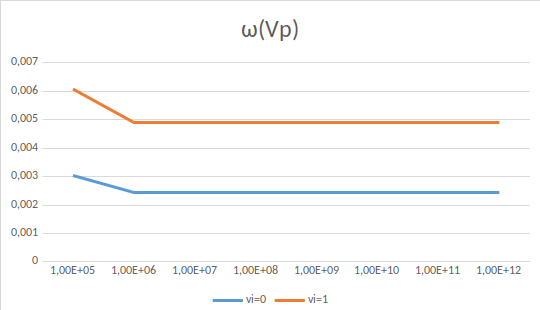
\includegraphics[scale=0.7]{img_5}}
	\caption{График зависимости $\omega(V_\rho)$ при $v_i = 0$ (нижняя) и $v_i = 1$ (верхняя)}
	\label{img:5}
\end{figure}

\begin{figure}[H]
	\renewcommand{\figurename}{Рисунок}
	\centering{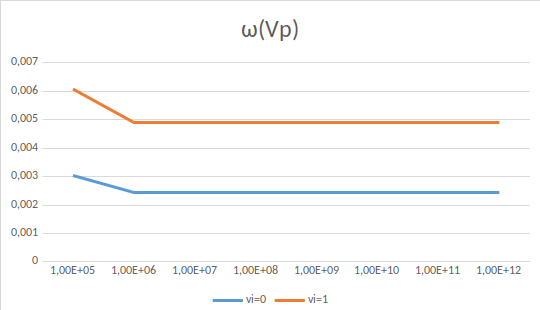
\includegraphics[scale=0.7]{img_5}}
	\caption{График зависимости $u(V_\rho)$ при $v_i = 0$ (нижняя) и $v_i = 1$ (верхняя)}
	\label{img:5}
\end{figure}


\newpage



